\section{Data sources}
\subsection{YouTube}
\subsubsection{YouTube data}
YouTube stores various data concerning its users and content. Tables
\ref{ut_video_info} - \ref{ut_channel_info} show the types of information
available.

\begin{table}[ht]
	\begin{tabular}{|p{3cm} | l | p{4cm}|}\hline
		Information & Access & Description\\ \hline

		Title & Public API & \\
		Published & Public API & \\
		Updated & Public API & \\
		Category & Public API & \\
		Tags (keywords) & Public API & \\
		Comments & Public API & \\
		Permissons & Public API & \\
		Description & Public API & \\
		Thumbnails & Public API & Set of video's thumbnails (along with times
		when taken) \\
		Duration & Public API & \\
		Ratings & Public API & Best, worst and average rating, number of votes \\
		Viewcount & Public API & \\
		Favourite count & Public API & \\
		Number of likes & Public API & \\
		Number of dislikes & Public API & \\
		Aspect ratio & Public API & \\
		Related & Public API & \\
		Responses & Public API & \\
		Author & Public API & \\ \hline
	\end{tabular}
	\caption{Information available for a video}
\end{table}

\begin{table}[ht]
	\begin{minipage}[b]{0.5\linewidth}
	\centering
		\begin{tabular}{ | p{3cm} | l |}\hline
		Information & Access \\ \hline
		Number of results & Public API \\
		Search results & Public API \\ \hline
		\end{tabular}
		\caption{Information available for video search results}
	\end{minipage}
	\hspace{0.5cm} % no new lines here!!
	\begin{minipage}[b]{0.5\linewidth}
		\centering
		\begin{tabular}{ | p{3cm} | l |}\hline
			Information & Access\\ \hline
			Uploads & Public API \\
			Gender & Public API \\
			Location & Public API \\
			Age & Public API \\
			Contacts & Public API \\
			Username & Public API \\
			Subscriptions & Public API \\
			Inbox & Public API \\
			Favorites & Public API \\
			History & Screen scraping \\
			Likes & Screen scraping \\
			Issued authentication subtokens & Screen scraping \\ \hline
		\end{tabular}
		\caption{Information available for a user}
	\end{minipage}
\end{table}


\begin{table}[ht]
	\begin{minipage}[b]{0.5\linewidth}\centering
		\begin{tabular}{ | p{3cm} | l |}\hline
			Information & Access \\ \hline
			Created & Public API \\
			Updated & Public API \\
			Author & Public API \\
			Text & Public API \\ \hline
		\end{tabular}
		\caption{Information available for a comment}
	\end{minipage}
	\hspace{0.5cm} % no new lines here!!
	\begin{minipage}[b]{0.5\linewidth}
		\centering
		\begin{tabular}{ | p{3cm} | l |}\hline
			Information & Access \\ \hline
			Demographics & Screen scraping \\
			Referrers & Screen scraping \\
			Countries popularity & Screen scraping \\ \hline
		\end{tabular}
		\caption{Information available for a channel}
	\end{minipage}
\end{table}


\subsubsection{YouTube usage}

A statistics were performed measuring popularity of three YouTube features: favourites,
subscriptions and uploads. Over a sample of 7500 users most settled down at
relatively low level of activity. All histograms below show numbers of users
(axis y) with $x_1-x_2$ numbers of favourites/subscriptions/uploads. For all
three cases, almost all users belonged to the first histogram range -- the one
with least items. As number of items grew, the number of users decreased so
quickly, that logarithmic scale must have been used in order to make charts
readable.

\begin{figure}[ht]
  \centering
  \subfigure[Favourites]{
		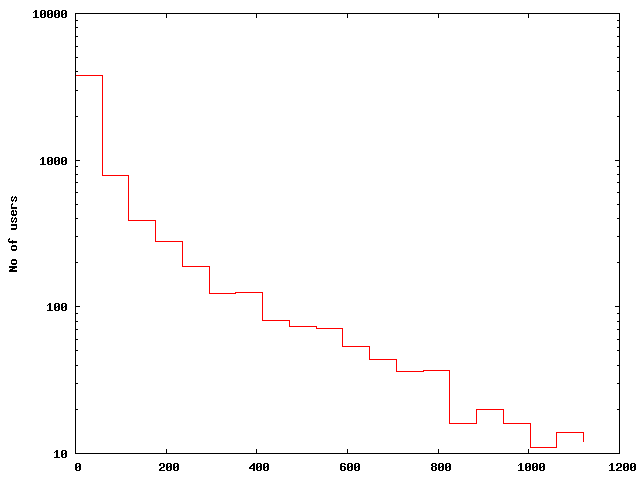
\includegraphics[scale=0.6]{images/favs.png}
		\label{fig:favs}
  }
  \subfigure[Subscriptions]{
		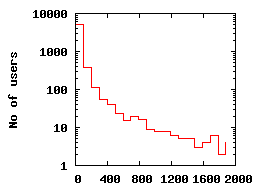
\includegraphics[scale=0.6]{images/subs.png}
		\label{fig:subs}
  }
  \subfigure[Uploads]{
		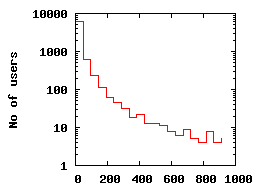
\includegraphics[scale=0.6]{images/ups.png}
		\label{fig:ups}
  }
  \label{fig:subfigureExample}
  \caption{Histograms of usage of favourites \subref{fig:favs}, subscriptions
  \subref{fig:subs} and uploads \subref{fig:ups}. The x axis represents groups of
  users having $x_1-x_2$ entities, the height of the bars indicates sizes of the
  groups.}
\end{figure}

\subsection{Vocabularies}
In order to make the user profile compatible with linked data sources, we used
vocabularies of semantic data from the freebase.com service. In particular --
entities connected to media: film and television actors, movies and television
shows titles, bands' and singers' names.

\subsection{Twitter}
\subsubsection{The Corpus}
The example data to be analyzed consists of Twitter streams of over 70 users
consisting in total of about 9000 tweets. They have been selected from the followers of most popular TV channels and broadcasters available on Twitter basing on the amounts of tweets they have accumulated, the amount of their followers and the language they are tweeting in (English in this evaluation).

The most significant reason for using a preselected corpus for this research is
the Twitter API Rate Limiting which makes a wider analysis challenging.
Furthermore, a great deal of Twitter users provide completely irrelevant
information or tweet in languages not useful for this research, which also
influences the effectiveness of a limited Twitter data aggregator. Using a preselected corpus enables measuring and comparing the effectiveness of different counting methods much easier.

\subsubsection{Types of messages}
\paragraph{Mentioning entities names}
Using trivial methods of string matching, Twitter data will be analyzed for
mentions of entities' names in tweets.
\\ Occurences of entity names a few times in a stream without a
provided activity or preference tag will most certainly indicate an interest in
the entity mentioned.
\\What is also interesting is the frequency of those mentions. Not only does
the total mentions count, but also the relative amount of tweets mentioning an
entity within all tweets.
\paragraph{Usage of preference verbs when tweeting about entities}
For extracting useful preference information, a vocabulary consisting of
popular preference verbs and adjectives is being used.
\\ As more data is gathered, the preference vocabulary is also being expanded
with verbs and adjectives referring to negative opinions on a subject.
\paragraph{Usage of activity verbs when tweeting about entities}
Describing the activity of participating in a certain TV experience (such
as watching a show) will also need to be marked as preferential due to the
fact that Twitter users are more likely to specify what they are doing at a
particular moment)
\paragraph{Researching the structure of the most popular mentions}
By retrieving tweets containing the entities, a ranking of most popular words
appearing with the entities will be created and by extracting the most useful
ones, the vocabularies will be updated.
\paragraph{Mentioning an entity as a hashtag}
witter users also use Hashtags for easier retrieval of tweets mentioning
a particular subject. When using a hashtag, all possible whitespace between
words naming an entity are removed and prefixed with a \# character.
\paragraph{Mentioning an entity via twitter username}
Provided we have a twitter username of an entity, it may be mentioned using
the Twitter mention system (using the @ character in front of the twitter
 username)
\paragraph{Extracting entities from structured twitter stream sources}
Some applications, such as YouTube of Boxee, can automatically generate tweets
if the user linked their Twitter account with that application. These tweets are
usually very well structured, and therefore very suitable to extract an entity, verb and/or rating from.
\paragraph{Mentioning and following entities}
Relate the mentions of entities followed (for known Twitter usernames) and the mentions of those and other entities. Mentioning can occur via:
\begin{itemize}
\item entity's name
\item entity's twitter username
\item entity converted to a hashtag form
\end{itemize}
\paragraph{Following preferenced entities}
Relating the sole fact of following an entity's twitter username and the preferences towards it based on other counting methods.

\subsubsection{Types of measurements available}
\begin{center}
  \begin{tabular}{ | p{4cm} | p{7cm} | } \hline
    \multicolumn{2}{|c|}{Types of measurements available} \\
    \hline
    \multirow{4}{*} {Mentioning entities}
      & Full name matching \\ \cline{2-2}
      & Matching the twitter username (if known) \\ \cline{2-2}
      & Matching the acronym (for names consisting of more than 3 words) \\ \cline{2-2}
      & Matching name converted to a hashtag form \\
    \hline
    Usage of activity verbs & Mentions using activity verbs \\
    \hline
    \multirow{3}{*}{Using preference verbs}
      & Mentions using preference verbs \\ \cline{2-2}
      & Positive preferences \\ \cline{2-2}
      & Negative preferences \\ \cline{2-2}
    \hline
    Structured streams & Extracting preference from generated tweets \\
    \hline
    \multirow{3}{*}{Following entity}
      & Mentioning the entity by name while following \\ \cline{2-2}
      & Relation between following and actual preferences \\ \cline{2-2}
    \hline
    \multirow{3}{*}{Researching mentions}
      & Statistics of words most used with mentions \\ \cline{2-2}
      & Finding average amount of mentions-to-tweets ratio \\ \cline{2-2}
    \hline
  \end{tabular}
\end{center}

\subsubsection{Results}
\paragraph{Diversing results}
In order for the results to actually bring any outcome, we decided to divide the
corpus into two halves. By measuring the
difference in achieved results, we might be actually able to evalute their
usefulness.

\paragraph{Full name matching}
Mentioning a full name (for all actors and also tv-shows/movies titles longer
than one word).

\begin{center}
  \begin{tabular}{ | p{4cm} | p{2cm} | p{1cm}| p{2cm} | } \hline
    Entity (average) & Corpus 1 & & Corpus 2 \\ \hline
    TV Shows & 1.24\% & & 1.76\% \\ \hline
    TV Actors & 0.41\% & & 0.00\% \\ \hline
    Movies & 1.92\% & & 1.69\% \\ \hline
    Movie actors & 0.74\% & & 0.21\% \\ \hline
  \end{tabular}
\end{center}

This score should be considered a baseline for further research. However, simple
mentioning a TV Show in somebody's stream most definitely is a sign of interest
(not necessarily preference) in the given subject.

\paragraph{Matching twitter usernames}
Since it is extremely hard to locate twitter usernames for some entities (such
as movies), that approach seems not to be useful. By picking up two twitter
usernames for two separate TV shows and adding them to the pool, we have noticed
extremely little (0.02\% in on of the corpuses for TV Shows) to almost none increase in search results.
However, the time needed for locating twitter usernames for those entities might
be too much compared to results that this method offers.

\paragraph{Matching title acronyms}
Only entities with a title with 3 or more words have been used for this
measurement.

\begin{center}
  \begin{tabular}{ | p{4cm} | p{2cm} | p{1cm}| p{2cm} | } \hline
    Entity (average) & Corpus 1 & & Corpus 2 \\ \hline
    TV Shows & 3.07\% & & 2.17\% \\ \hline
    Movies & 2.01\% & & 2.33\% \\ \hline
  \end{tabular}
\end{center}

We can easily spot an increase in matched entities, however there might be many
misleading acronyms created with this approach. Acronyms such as \textit{SNL}
(for \textit{Saturday Night Live} show) or  \textit{BBT} (\textit{Big Bang
Theory}) are widely used, probably even as much as the full titles. However,
if a \textit{CAT} acronym emerges, it will drastically reduce the effectiveness
of matching algorithms.

\paragraph{Matching name converted to a hashtag form}
All entities have been converted to a hashtag form (such as
\textit{\#SaturdayNightLive} for Saturday Night Live). Also one-word entity
names have been used.

\begin{center}
  \begin{tabular}{ | p{4cm} | p{2cm} | p{1cm}| p{2cm} | } \hline
    Entity (average) & Corpus 1 & & Corpus 2 \\ \hline
    TV Shows & 1.48\% & & 2.21 \% \\ \hline
    TV Actors & 0.11\% & & 0.03\% \\ \hline
    Movies & 2.49\% & & 3.12\% \\ \hline
    Movie actors & 0.67\% & & 0.19\% \\ \hline
  \end{tabular}
\end{center}

We can easily notice how the person-based entities have either noted a smaller
occurence rate and title-based ones have improved. This may be related to the
fact that people usually create hashtags based on a more general entity (such as
    a movie) rather then specific it's parts (such as actors that play in it)
when expressing their opinion.

\paragraph{Usage of activity verbs}
Not a great set of activity verbs has been used. Verbs like \textit{watch},
\textit{view}, \textit{see}, \textit{catch} and their past forms are
amongst them. \\
Below is a figure showing percentage of tweets using an activity verb
and a entity name (full match).

\begin{center}
  \begin{tabular}{ | p{4cm} | p{2cm} | p{1cm}| p{2cm} | } \hline
    Entity (average) & Corpus 1 & & Corpus 2 \\ \hline
    Movies & 37.4\% & & 24.3\% \\ \hline
    TV Shows & 21.2\% & & 13.4\% \\ \hline
    TV Actors & 1.3\% & & 0.6\% \\ \hline
    Movie actors & 2.1\% & & 0.0\% \\ \hline
  \end{tabular}
\end{center}

As we can see, the activity verbs are very unlikely to be occuring next to
person-based entities. However, activity verbs are much more popular with both
Movies and TV Shows, which originates from the very idea of Twitter and
updating statuses with information on what the user is currently doing.

\paragraph{Usage of preference verbs}
Two sets of preference have been used:
\begin{itemize}
\item positive
\item negative
\end{itemize}

The figure below shows the general use of preference verbs with occurences of
mentions.

\begin{center}
  \begin{tabular}{ | p{4cm} | p{2cm} | p{1cm}| p{2cm} | } \hline
    Entity (average) & Corpus 1 & & Corpus 2 \\ \hline
    TV Shows & 7.4\% & & 6.3\% \\ \hline
    Movies & 9.1\% & & 8.4\% \\ \hline
    TV Actors & 0.0\% & & 0.9\% \\ \hline
    Movie actors & 1.2\% & & 2.7\% \\ \hline
  \end{tabular}
\end{center}

And a positive-to-negative preference ratio:

\begin{center}
  \begin{tabular}{ | p{3cm}| p{2cm} | } \hline
    Type & Amount \\ \hline
    Positive & 92\% \\ \hline
    Negative & 8\% \\ \hline
  \end{tabular}
\end{center}

The amount of preference verbs used whilst mentioning an entity is definitely
smaller compared to activity verbs. However, the Positive-to-Negative ratio most
certainly suggests that users' media preferences expressed on Twitter are
usually positive.

\paragraph{Relation between preferences and following}
By gathering available Twitter usernames from the \textit{Freebase} database,
we were able to perform searches for mentions of those usernames within the followers' streams.

The following figure shows the share of different kind of mentions of the specific entity while following.

\begin{center}
  \begin{tabular}{ | p{3cm}| p{2cm} | } \hline
    Match type & Occurence \\ \hline
    Name & 0\% \\ \hline
    Hashtag & 6\% \\ \hline
	Username & 94\% \\ \hline
  \end{tabular}
\end{center}

Since Twitter usernames mostly represent specific people rather than any other kinds of entities, it seems as if users mostly
refer/mention them using their usernames rather than their names in plain or hashtag form.

However, those mentions occur relatively rarely. For a sample of 70 twitter usernames and 5 followers each
(around 4000 tweets), we were able to find out only 24 tweets (about 0.57\%) mentioning directly the people they are following.

Furthermore, following a certain entity should also be regarded as a preference toward the topics this entity is connected to (such as
Politics for \textit{BarackObama}).

On the other hand, locating more \textit{official} twitter usernames for various entities might be extremely hard,
making this approach not completely worthwhile. Given such small amounts of twitter usernames known, it would be
hard to reasonably specify the relation between the act of following the entity on twitter and preferences
towards it, thus making in the profiling based on the ones known less influential as the other methods.

\subsubsection{Summary}
All the methods used are slightly naive and may not always reflect the actual
state of preferences. Not only do some names of entities not actually always
represent what we would like them to. Due to a very specific nature of the
tweets, it is quite hard to apply more definite Natural Language Processing
methods. Tweets mostly do not contain a proper object making it quite hard to
relate the activity/preference verb to the entity itself.
